%%==================================================
%% abstract.tex for BIT Master Thesis
%% Edited by Jian dahao
%% version: 1.0
%% last update: May 10th, 2019
%%==================================================
\chapter{数学公式使用}
数学公式的使用可先参考官方模板中的BIT-Thesis使用指南。
\section{公式编辑}
LaTeX公式是通过代码的形式进行编辑,运算符号、特殊字母等数学符号对应的命令可参考链接\url{http://www.mohu.org/info/symbols/symbols.htm}。不会写代码或者不想敲代码怎么办,可以通过MathType、LaTeX公式在线编辑工具等进行编辑,然后导出tex代码。
\subsection{用MathType编辑}
首先你需要一个已经破解的MathType工具。打开MathType后在设置剪切复制选项。
\begin{figure}[h]
\centering
 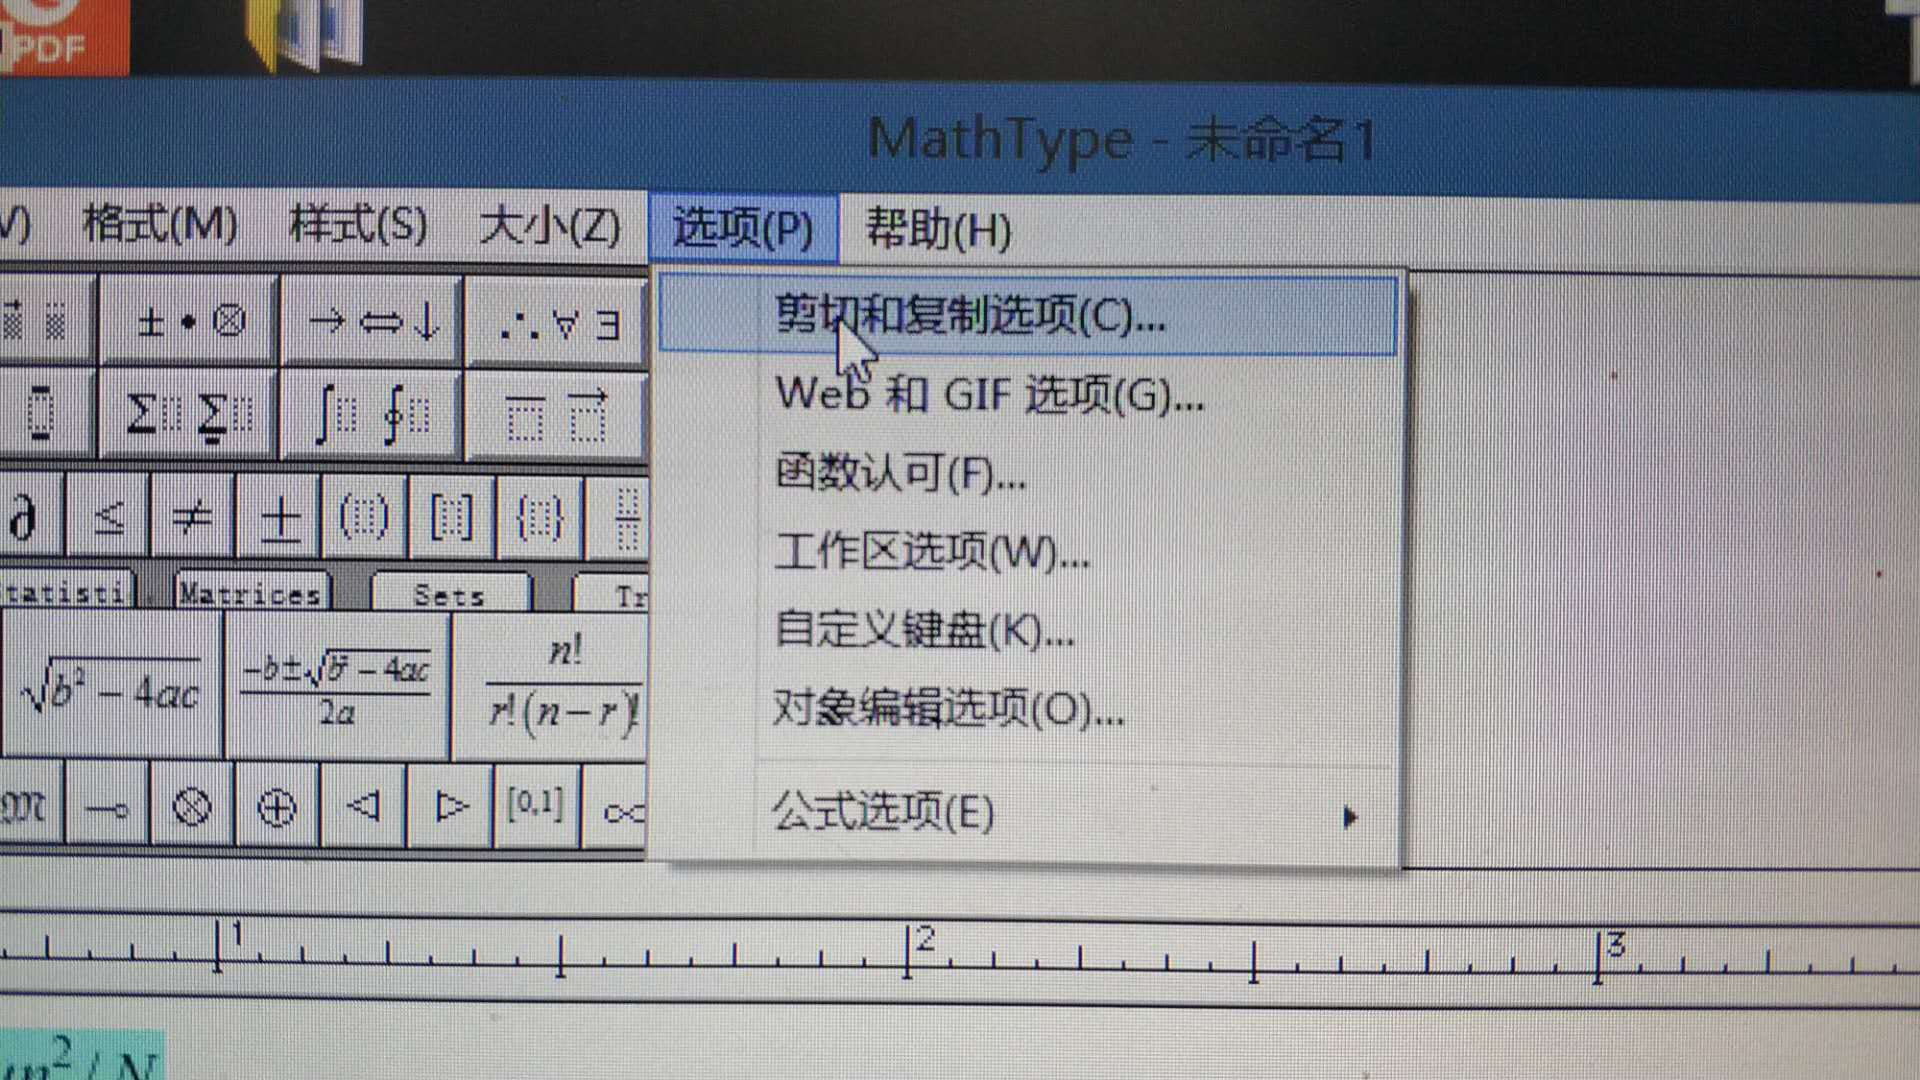
\includegraphics[width=0.75\textwidth]{chapters/figures/mathtype_copy_type.jpg}
\end{figure}
然后在\textbf{转换其他文字}中选择\textbf{Plain Tex}或者\textbf{LaTeX 2.09 and later},诸如此类即可。

用MathType编辑好公式后,只需全选复制或剪切就能获得公式代码,例如公式
\begin{equation}
A(n) = e^{4j\pi \mu n^2/N} \notag
\end{equation}
对应的导出结果为:\\
% \begin{lstlisting}[language={tex}, caption={插入公式基本操作}]
Plain Tex:\textbf{\$\$}A(n)\{\rm\{ = \}\}\{e\^\ \{4j$\backslash$pi $\backslash$mu \{n\^\ 2\}/N\}\}\textbf{\$\$} \\
Latex 2.09 and later: $\backslash$[A(n)\{$\backslash$rm\{ = \}\}\{e\^\ \{4j$\backslash$pi $\backslash$mu \{n\^\ 2\}/N\}\}$\backslash$]

需要注意的是,导出的tex代码中需要删除对应的前缀和后缀:对于\textbf{Plain Tex}为\$\$;对\textbf{Latex 2.09 and later}为$\backslash$[ $\quad$ $\backslash$]。

\begin{figure}[h]
\centering
 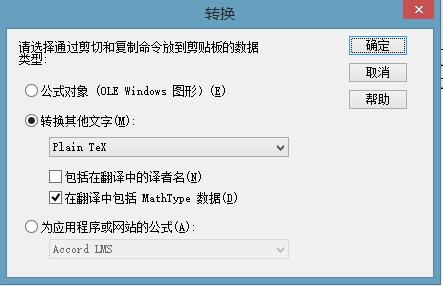
\includegraphics[width=0.75\textwidth]{chapters/figures/copy_type.jpg}
\end{figure}
\subsection{用在线工具编辑}
推荐两个网站

\url{http://latex.codecogs.com/eqneditor/editor.php}

\url{https://www.codecogs.com/latex/eqneditor.php}

个人还是比较推荐学一下基本的tex公式语法(边用边学就好),这样写起来会快很多。

\section{怎么插入公式}
% \subsection{段落间插入公式}
对于插入到段落之间的且需要编号公式其定义的内容需要被包含在$\backslash$begin\{equation\}$\backslash$end \{equation\} 之间,基本使用方法如下:
\begin{lstlisting}[language={tex}, caption={插入公式基本操作}]
\begin{equation}
A(n) = e^{4j\pi \mu n^2/N}
\end{equation}
\end{lstlisting}
插入效果为:
\begin{equation}
A(n) = e^{4j\pi \mu n^2/N}
\end{equation}
% \subsection{文本中插入公式}
而对于插入到文本中间的公式只需将公式内容用一对\$\$包起来即可,例如:
这是一段文本这里要插入的公式用法为\$2\^\ \{n\}\$,对应的效果为$2^{n}$。
\section{公式换行与跨页}
由于经常会遇到插入的数学公式巨长,无法在一行上正常显示,或者为了排版美观而需要进行强制换行,常用方法如下。
\subsection{公式换行之基本操作}
\label{sec:公式换行之基本操作}
\vspace{-1cm}
\begin{lstlisting}[language={tex}, caption={结合split和equation环境插入公式}]
\begin{equation}
\begin{split}
A(n) &= e^{4j\pi \mu n^2/N} \\
&= e^{4j\pi \mu n^2/N}
\end{split}
\end{equation}
\end{lstlisting}
其中\&代表对齐位置,$\backslash\backslash$代表换行。对应的插入效果为:
\begin{equation}
\begin{split}
A(n) &= e^{4j\pi \mu n^2/N} \\
&= e^{4j\pi \mu n^2/N}
\end{split}
\end{equation}
\subsection{公式想换行又跨页}
\label{sec:公式想换行又跨页}
\vspace{-1cm}
\begin{lstlisting}[language={tex}, caption={使用align环境插入公式}]
\begin{align}
A(n) &= e^{4j\pi \mu n^2/N} \notag\\
&= e^{4j\pi \mu n^2/N} \notag\\
&= e^{4j\pi \mu n^2/N}
\end{align}
\end{lstlisting}
其中$\backslash$notag用于指定该行代码不被编号,$\backslash\backslash$和\&同样分别代表换行和对齐。效果为:
\begin{align}
A(n) &= e^{4j\pi \mu n^2/N} \notag\\
&= e^{4j\pi \mu n^2/N} \notag\\
&= e^{4j\pi \mu n^2/N}
\end{align}

\ref{sec:公式换行之基本操作}和\ref{sec:公式想换行又跨页}介绍的方法都可以实现公式的多行显示,但是第一种方法不支持公式的跨页显示。

\subsection{公式太长一行放不下}
有时数学公式比较复杂,无法在一行上完整显示一个表达式,一般情况下使用上述两种方法(\ref{sec:公式换行之基本操作}和\ref{sec:公式想换行又跨页}介绍的方法)即可解决,但是对于需要分行显示的公式被一对大尺寸括号(参见\ref{sec:如何插入大尺寸括号}内容)包括的情况则会编译出错或显示效果不佳,解决方法如下。假设处理的公式为:
\begin{equation}
P = \left(\sum_{n=1}^{N}It\ is\ a\ loooooooooooooooooooooooooooooooooooooooooooooooooooooooooog\ equation\right)
\end{equation}
通常有两种解决方案:\\
\textbf{1.使用$\backslash$left(和$\backslash$right)等自适应定界符拆分}\\
将长公式拆分成$\backslash$left(            $\backslash$right.     $\backslash$$\backslash$     $\backslash$left.     $\backslash$right)的形式,例如:
\begin{lstlisting}[language={tex}, caption={}]
\begin{equation}
\begin{split}
%也可以使用align环境
P = \left( \sum_{n=1}^{N}It\ is\ a\ looooooooooooooooooooooooooooooo\right. \\
\left. ooooooooooooooooooooooooooog\ equation \right)
\end{split}
\end{equation}
\end{lstlisting}
显示效果为:
\begin{equation}
\begin{split}
%也可以使用align环境
P = \left( \sum_{n=1}^{N}It\ is\ a\ looooooooooooooooooooooooooooooo\right. \\
\left. ooooooooooooooooooooooooooog\ equation \right)
\end{split}
\end{equation}
使用$\backslash$left(和$\backslash$right)等自适应定界符的好处是能够自动确定定界符的尺寸发小,但是这种方法可能出现如上面公式所示的情况:即虽然成功拆分了公式,但是两行的括号大小出现不一致的情况。所以对于这种情况,可以使用下面的方法来解决。\\
\textbf{2.使用规定大小的定界符来辅助拆分}\\
使用$\backslash$big,$\backslash$Big,$\backslash$bigg,$\backslash$Bigg等标签来辅助拆分,例如
% \begin{equation}
% \begin{split}
\begin{lstlisting}[language={tex}, caption={}]
\begin{equation}
\begin{split}
%也可以使用align环境
P = \Bigg( \sum_{n=1}^{N}It\ is\ a\ looooooooooooooooooooooooooooooo  \\
ooooooooooooooooooooooooooog\ equation \Bigg)
\end{split}
\end{equation}
\end{lstlisting}
\begin{equation}
\begin{split}
%也可以使用align环境
P = \Bigg( \sum_{n=1}^{N}It\ is\ a\ looooooooooooooooooooooooooooooo  \\
ooooooooooooooooooooooooooog\ equation \Bigg)
\end{split}
\end{equation}

\section{如何引用公式}
添加$\backslash$label{},即
\begin{lstlisting}[language={tex}, caption={添加公式标签}]
\begin{equation}
\label{equ:示例公式标签}
A(n) = e^{4j\pi \mu n^2/N}
\end{equation}
\end{lstlisting}
\begin{equation}
\label{equ:示例公式标签}
A(n) = e^{4j\pi \mu n^2/N}
\end{equation}
在引用处调用\textbf{$\backslash$ref\{equ:示例公式标签\}}即可$\to$\ref{equ:示例公式标签}
\section{如何插入大尺寸括号}
\label{sec:如何插入大尺寸括号}
在latex下编辑公式时,经常会用到各种括号。如果直接输入括号(花括号需要进行转义),其大小是固定的,如果公式的高度比较大,就会显得很不协调。另外,在括号中换行的话有可能会导致两行的左右括号大小不一致,影响美观。

\textbf{方法一:使用$\backslash$left 和 $\backslash$right}\\
$\backslash$left 放在左边括号前面,$\backslash$ight 放在右边括号前面,需要配对使用。该方法能自动控制不同层次括号的大小。
需要注意的是在对单括号使用 $\backslash$left和 $\backslash$right命令时,也需要配对使用,没有括号的一端要加点。
比如对左括号进行操作,命令如下:

$\backslash$left[.........$\backslash$right.

\textbf{方法二使用$\backslash$big 系列标签}\\
该系列标签包括$\backslash$big,$\backslash$Big,$\backslash$bigg,$\backslash$Bigg。按着顺序,它们控制的括号不断变大。不需要成对使用,可以单独控制半个括号
括号的大小由具体使用的标签控制,不能自动调整,所以需要注意匹配。例: 

$\backslash$big[............$\backslash$big]

\noindent\fbox{$\bigstar$:\textbf{一般情况下使用$\backslash$left\ $\backslash$right 就足够了。特殊情况下,比如公式换行才需要用到$\backslash$big}}
\section{自查重模式下如何关闭公式显示}
在模板BIT-thesis-LaTex中(使用BIT-thesis-grd-jdh.cls格式控制文件)可以使用$\backslash$insertEquation或者$\backslash$insertContents命令来实现。
\begin{lstlisting}[language={tex}, caption={}]
\insertEquation{
	\begin{equation}
		.......
	\end{equation}
}
\insertContents{
	\begin{equation}
		.......
	\end{equation}
}
\insertEquation{$E=mc^2$
\end{lstlisting}